\documentclass{alt2027}
\jmlrworkshop{38th International Conference on Algorithmic Learning Theory}
\usepackage{times,booktabs}
\hypersetup{hidelinks}
\title[Mario Level Memorization]{Midterm Progress Report (Track D, implementation-based):\\Do Generative Level Models Copy Their Training Data?}
\altauthor{\Name{Sujal Shrestha} \Email{sujalshrestha@ou.edu}\\
\Name{Jackson McKay} \Email{jackson.j.mckay-1@ou.edu}\\
\addr CS 4713, Fall 2026\\
Github: \url{https://github.com/sujalstha/MarioGPT}}
\begin{document}
\maketitle
\begin{abstract}
A playable generated Mario level may resemble a training level. We ask how often small Transformer and diffusion generators produce near-copies, and whether copying decreases as the training set grows. We trained 50 models on matched subsets of 3, 6, 9, 12, or 15 levels, with five seeds per setting, and generated 1,000 slices per model. At three levels, mean near-copy rates were 25.5\% for the Transformer and 23.9\% for diffusion. These are measurements from short, fixed training budgets rather than converged reproductions. Low copying alone cannot establish generalization: our held-out baseline and local reachability check help distinguish novelty from poor generation.
\end{abstract}
\begin{keywords}Track D, theory of modern AI; implementation-based study; memorization, level generation\end{keywords}
\section{Introduction}
Our proposal compares MarioGPT \citep{mariogpt}, a DistilGPT2-based tile generator, with the attention-equipped U-Net diffusion generator of \citet{diffusion}. Both evaluate playability with an A* agent. MarioGPT already examines memorization in Section 4.3 through nearest-training examples and sampling temperature. We extend that question with a quantitative copy threshold and a matched training-set-size sweep.

Our hypothesis is that more than half the outputs are near-copies at three training levels, and that copying falls as data increases. This tests overfitting behavior rather than proving a generalization bound.

\section{Implementation and Results}
\textbf{Setup.} We use 37 VGLC maps from Super Mario Bros. and The Lost Levels. Five whole levels are held out before extracting $14\times16$ slices (stride 1); maps are ground-aligned by cropping or padding above. Five seeds give nested subsets $k\in\{3,6,9,12,15\}$ shared by both architectures. Each of the $2\times5\times5=50$ models generates 1,000 slices. The private repository records data IDs, settings, outputs, and losses; \texttt{mlciv} has been invited.

The Transformer retains pretrained DistilGPT2 blocks with a tile vocabulary, omitting prompts and novelty search. It trains 300 updates with AdamW ($5\times10^{-5}$, zero weight decay), sampling at temperature 1 without top-$k$ truncation. Our 32/64/32-channel U-Net omits attention, training 1,500 updates with Adam ($10^{-3}$) on noise-prediction MSE. It uses 100 linear-beta DDPM steps ($10^{-4}$ to $0.1$) and argmax decoding. Both use batch 16. These are small adaptations; the diffusion paper uses $14\times14$ slices. Budgets are fixed across dataset sizes within each architecture.

\textbf{Experiment Set 1: copying.} We compute exact nearest-training Hamming distance, $d_{\min}(x)=\min_{s\in S}\sum_{i=1}^{224}\mathbf1[x_i\ne s_i]$. Near-copies have $d_{\min}\le11$ (at most 5\% of tiles); exact copies have distance zero. Table~\ref{tab:results} and Figure~\ref{fig:metrics} show results across five training runs per setting. Held-out real slices provide a baseline because larger training corpora offer more possible matches. Generated outputs are not independent training repeats.

\begin{table}[t]
\centering\small
\caption{Near-copy rate (\%): mean $\pm$ sample standard deviation over five seeds. The held-out baseline is shared by both architectures.}\label{tab:results}
\begin{tabular}{rrrr}\toprule
Training levels & Transformer & Diffusion & Held-out real slices\\\midrule
3 & 25.5 $\pm$ 12.8 & 23.9 $\pm$ 13.8 & 27.9 $\pm$ 3.1 \\
6 & 32.4 $\pm$ 19.4 & 23.3 $\pm$ 10.3 & 35.7 $\pm$ 1.8 \\
9 & 29.4 $\pm$ 11.0 & 38.9 $\pm$ 26.4 & 37.7 $\pm$ 2.5 \\
12 & 40.0 $\pm$ 14.9 & 37.8 $\pm$ 29.5 & 39.2 $\pm$ 3.0 \\
15 & 31.1 $\pm$ 6.7 & 29.8 $\pm$ 22.0 & 40.7 $\pm$ 2.5 \\
\bottomrule\end{tabular}
\end{table}

\begin{figure}[t]\centering
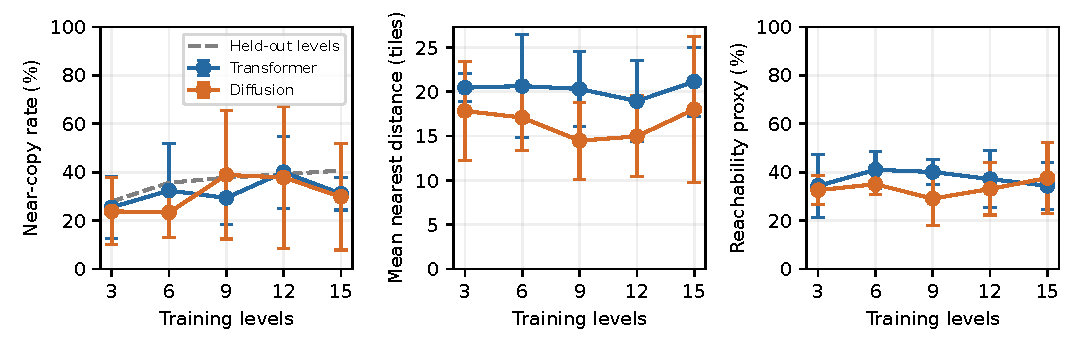
\includegraphics[width=\linewidth]{../figures/metrics.pdf}
\caption{Copy rate, nearest-training distance, and local reachability versus training-set size. Error bars show sample standard deviation over five seeds. The dashed curve is the held-out real-level baseline.}\label{fig:metrics}
\end{figure}

\textbf{Experiment Set 2: filtering.} A point-agent search tests left-to-right reachability using supported landing positions and approximate jump arcs (horizontal range and height up to four tiles). Enemies block traversal. We repeat the check on non-copied outputs. This is a local proxy, not Mario physics or full-level A* playability. Figure~\ref{fig:examples} shows minimum-distance outputs at $k=3$, seed 0.

\begin{figure}[t]\centering
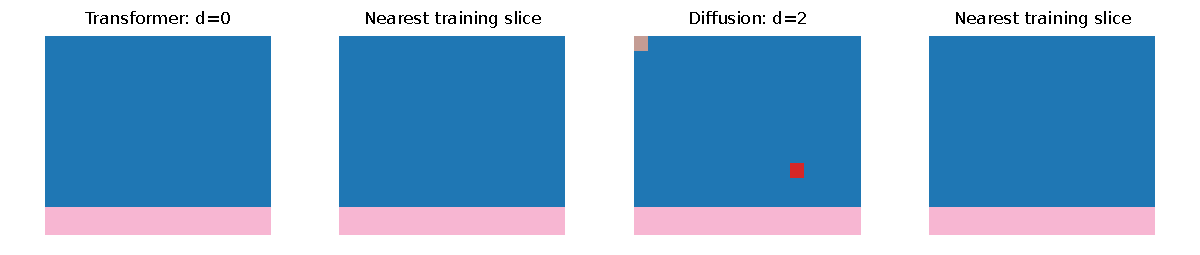
\includegraphics[width=.88\linewidth]{../figures/examples.pdf}
\caption{Closest generated/training pairs ($k=3$, seed 0). Blue is empty space; pink is solid X blocks. Common ground-and-sky patterns can match exactly.}\label{fig:examples}
\end{figure}

Transformer: mean reachability 37.4\% before filtering and 35.4\% after; exact-copy rate 1.0\%. Diffusion: mean reachability 33.5\% before filtering and 37.0\% after; exact-copy rate 0.0\%. Means weight the 25 runs equally. Both three-level mean copy rates are below our hypothesized 50\%, and neither curve decreases monotonically. Short training and unequal capacities limit interpretation: low copying does not establish useful generalization.

\section{Difficulties So Far}
\begin{itemize}\setlength{\itemsep}{0pt}
\item \textbf{Data:} Lost Levels supplements the 15-map base corpus; mixed heights require normalization.
\item \textbf{Compute:} The workflow used 17:12 GPU-minutes (cap: 45). These short runs do not establish convergence.
\item \textbf{Evaluation:} Common patterns inflate matches. Hamming boundary and simple reachability tests passed; all saved distances were recomputed.
\end{itemize}

\section{Plan for the Rest of the Semester}
\begin{itemize}\setlength{\itemsep}{0pt}
\item \textbf{Nov. 10--25:} Check convergence with longer training, vary sampling temperature, and improve playability evaluation on the same splits.
\item \textbf{Nov. 26--Dec. 7:} Relate copying to training exposure, capacity, and overfitting.
\item \textbf{Dec. 8/10; Dec. 14:} Present, then submit the final report and code. The required 15-minute meeting with Dr. Cao remains to be scheduled and completed.
\end{itemize}

\section{What Each of Us Has Done}
\textbf{Sujal Shrestha:} Supplied the team proposal and directed scope and compute budget. \textbf{Jackson McKay:} No completed individual technical contribution was reported. \textbf{AI assistance:} Codex implemented and ran experiments, generated figures, and drafted this report. Both students still need to review the code, results, and paper connections.

\begin{thebibliography}{2}
\bibitem[Sudhakaran et~al.(2023)]{mariogpt} S. Sudhakaran, M. Gonz\'alez-Duque, M. Freiberger, C. Glanois, E. Najarro, and S. Risi. MarioGPT: Open-Ended Text2Level Generation through Large Language Models. \emph{NeurIPS}, 2023.
\bibitem[Lee and Simo-Serra(2023)]{diffusion} H. J. Lee and E. Simo-Serra. Using Unconditional Diffusion Models in Level Generation for Super Mario Bros. \emph{MVA}, 2023.
\end{thebibliography}
\end{document}
